\section{Charm production}
\label{sec:charm}

Following the discussion of inclusive DIS observables in the previous section, we move to study charm production; see Sect.~\ref{sec:settings} for the charm-tagging definition adopted.
%
For this charm-production analysis we use somewhat tighter fiducial cuts, namely $Q^2>4$~GeV$^2$ and $W>5$~GeV  instead of Eq.~(\ref{eq:fiducial}) to account for the larger typical invariant mass of the hadronic final state in this subprocess. 

\paragraph{Fiducial cross-sections.}
%
Fig.~\ref{fig:charm-vs-energy} displays the same comparison as Fig.~\ref{fig:sigma-vs-energy} now for inclusive charm production.
%
For neutrino DIS, we also display the predictions of \powhegtwo for which we allow a non-zero value of the charm mass, $m_c\ne 0$, which are denoted by \powhegtwomc in the following.
%
To benchmark the latter, we also consider here the \yadism calculation in the FFNS $n_f=3$ scheme, with no charm in the proton, which corresponds to the same heavy-quark mass scheme as that adopted in the \powhegtwomc predictions.

%%%%%%%%%%%%%%%%%%%%%%%%%%%%%%
\begin{figure}[!tbp]
  \centering
  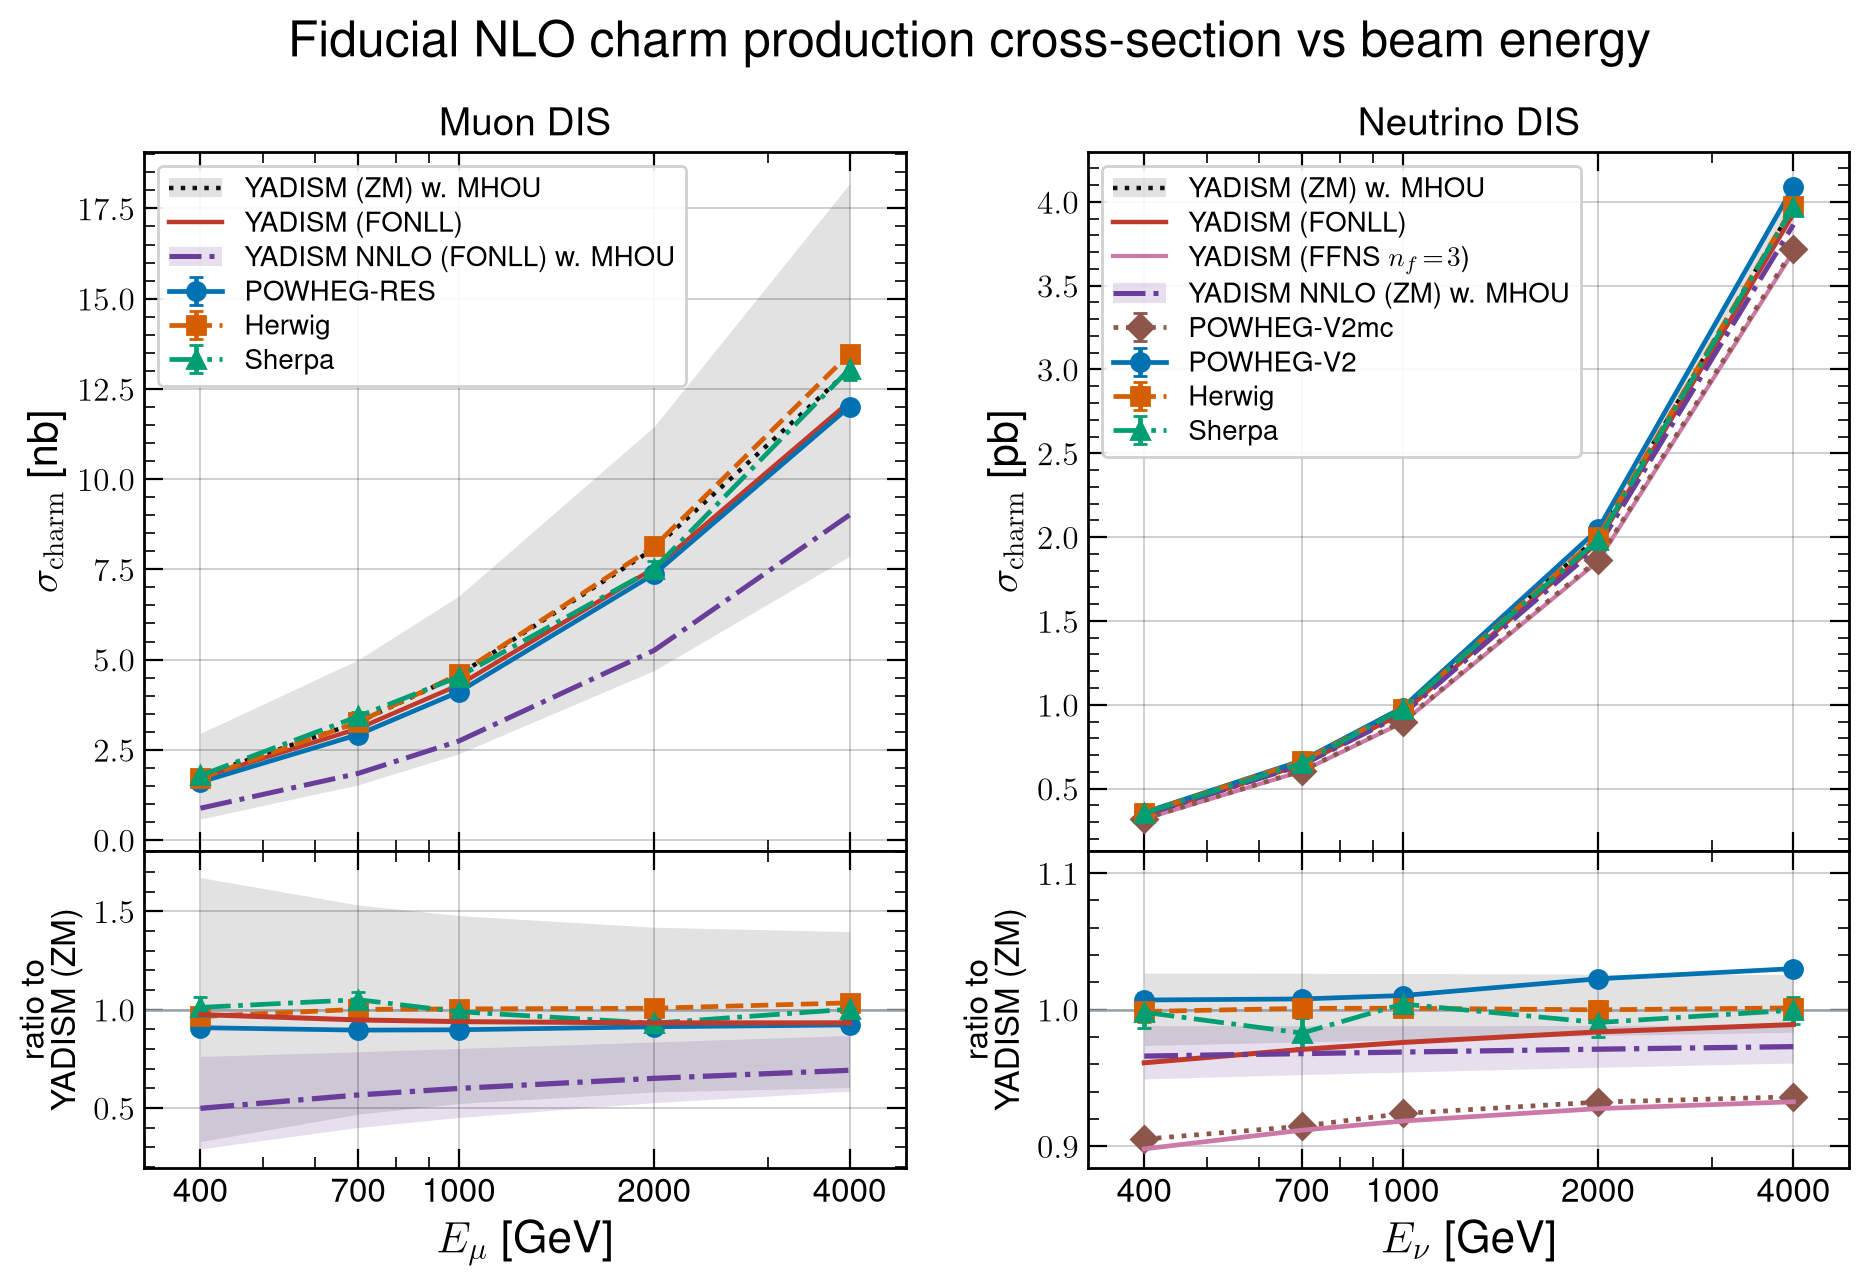
\includegraphics[width=0.99\textwidth]{figures/pp_charm_vs_energy.png}
  \caption{Same as Fig.~\ref{fig:sigma-vs-energy} now for inclusive charm production in the fiducial region with $W>5$~GeV; see Sect.~\ref{sec:settings} for the charm-tagging definition.
%
For neutrino DIS, we also display the predictions of \powhegtwo for which $m_c\ne 0$ (\powhegtwomc), together with the \yadism calculation in the FFNS $n_f=3$ scheme, which matches the mass scheme of \powhegtwomc.
}
  \label{fig:charm-vs-energy}
\end{figure}
%%%%%%%%%%%%%%%%%%%%%%%%%%%%%%%%%%%

From Fig.~\ref{fig:charm-vs-energy} we observe that the three NLO-matched generators agree with the \yadism ZM NLO reference within a few per cent for neutrino DIS and within about $10\%$ for muon DIS, with residual differences largely covered by the MHOU band of the NLO calculation.
%
Charm quark mass effects in the matched calculation can be estimated from the shift between the ZM-VFNS and FONLL 
\yadism predictions and amount to $3$--$7\%$ for muon DIS and to $1$--$4\%$ for neutrino DIS, in the latter case comparable to the magnitude of the NLO MHOU band.

Charm mass effects at the event generator level in neutrino DIS are quantified by comparing \powhegtwomc with \powhegtwo, with the former lying $8$--$10\%$ below the latter depending on the value of $E_\nu$.
%
\powhegtwomc does not resum potentially large logarithms $\ln(Q^2/m_c^2)$ encoded in the charm PDF as the FONLL calculation does, and hence it may underestimate the charm-production cross-section.
%
The \powhegtwomc prediction agrees closely with the corresponding \yadism calculation in the same mass scheme (FFNS $n_f=3$).
%
The spread between purely massive, massless, and matched calculations in the right panel of Fig.~\ref{fig:charm-vs-energy} emphasises the importance of carefully accounting for heavy-quark mass effects in predictions for charm production in DIS event generation.  

Fig.~\ref{fig:charm-vs-energy} also indicates that the perturbative behaviour of NC and CC predictions is quite different.
%
For neutrino DIS, the NNLO correction to the charm cross-section is at most $-3\%$ at every energy, and the size of the MHOUs is reduced from about $2.5\%$ at NLO to $1.5$--$2\%$ at NNLO.
%
We note however that this comparison is carried out at the purely massless level, and accounting for mass effects in the FONLL matched calculation extended to NNLO may modify this conclusion.
%
For charm production in muon DIS instead, the perturbative series converges slowly, with NNLO corrections being as large as $-50\%$, though a marked reduction of the associated MHOU band is also observed at the highest energies. 
%
This slow convergence follows from the low-$Q^2$ behaviour of the charm coefficient functions near threshold, driven by the $Q^{-4}$ enhancement of the photon propagator which pins the neutral-current rate against the $Q^2$ cut at every beam energy.
%
As for the inclusive DIS case discussed in Sect.~\ref{sec:inclusive}, a significant improvement of the perturbative convergence of charm production is observed by raising the $Q^2$ cut above $4$~GeV$^2$.
%
For instance, for $Q^2>11$~GeV$^2$ the NNLO/NLO ratio of the muon charm cross-section increases from $0.51$--$0.74$ to $0.78$--$0.86$ in the considered energy range, while the size of the MHOUs, at most $47\%$ at both NLO and NNLO for $Q^2>4$~GeV$^2$, is reduced to $24\%$ at NLO and to $16\%$ at NNLO, the largest values being found at $E_\mu=400$~GeV.

Fig.~\ref{fig:genie-charm-vs-energy} compares the NLO \yadism (FONLL and FFNS $n_f=3$) and \powheg calculations of charm production in neutrino DIS shown in Fig.~\ref{fig:charm-vs-energy} with those from \genie for the same configurations considered  in  Fig.~\ref{fig:genie-vs-energy}.
%
The default \genie tune (GRV98LO) lies about $40\%$ below the FONLL reference, a deficit which is mostly related to the choice of PDFs and in particular to the shape and magnitude of the strange sea PDF. 
%
Indeed, substituting \nnpdf for GRV98 within the same \genie tune results in a prediction in agreement with the \yadism FONLL reference. 
%
The NLO {\sc\small HEDIS} tune also predicts a suppression of up to 15\% as compared to the reference, also explained by PDF differences as was the case for inclusive cross-sections in Sect.~\ref{sec:inclusive}.
%
This PDF sensitivity emphasises that FASER neutrino DIS data provide a powerful probe of the strange content of the nucleon, as we further quantify in Sect.~\ref{sec:faser-app}.

%%%%%%%%%%%%%%%%%%%%%%%%%%
\begin{figure}[!tbp]
  \centering
  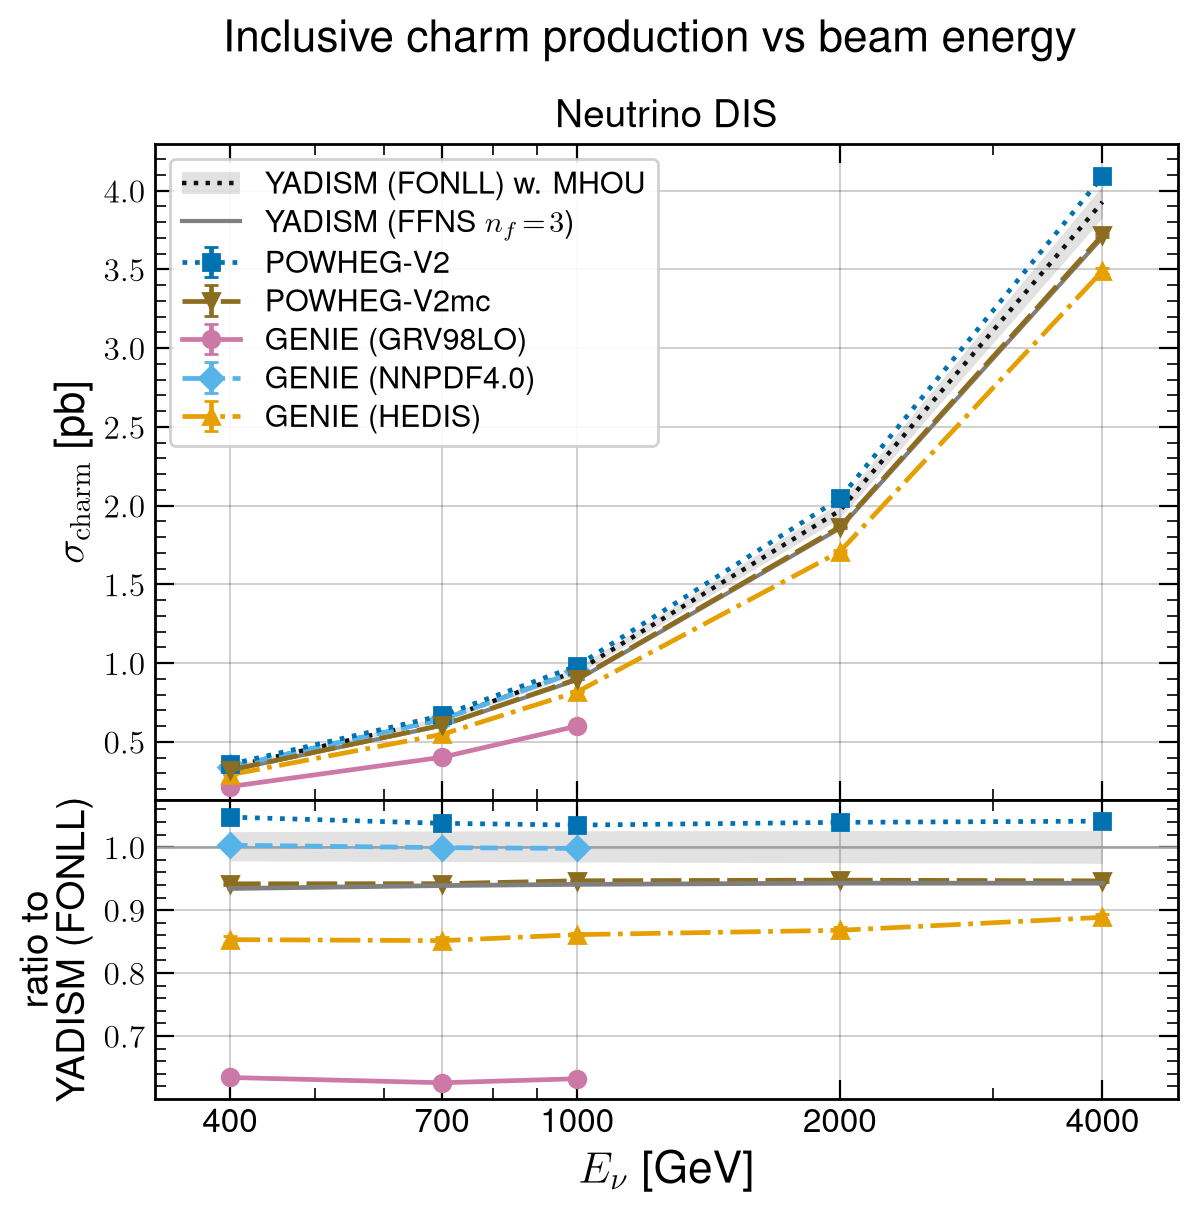
\includegraphics[width=0.7\textwidth]{figures/pp_genie_charm_vs_energy.png}
  \caption{Same as Fig.~\ref{fig:charm-vs-energy}, comparing the NLO \yadism (FONLL and FFNS $n_f=3$) and \powheg calculations of charm production in neutrino-induced DIS with those from \genie for the same configurations considered  in  Fig.~\ref{fig:genie-vs-energy}.
    %
    The bottom panels display the ratio to the \yadism FONLL prediction.
    }
  \label{fig:genie-charm-vs-energy}
\end{figure}
%%%%%%%%%%%%%%%%%%%%%%%%%%%%

\paragraph{Charm fragmentation.}
%
The fact that the various NLO event generators considered in Fig.~\ref{fig:charm-vs-energy} agree at the charm-tagged cross-section level when a common set of input settings is adopted does not necessarily imply that they all predict the same pattern of charm fragmentation into different $D$-meson species. 
%
To assess this feature, Fig.~\ref{fig:dmeson-ratios} displays the ratios $\langle N_{D^\pm}\rangle/\langle N_{D^0}\rangle$ and $\langle N_{D_s^\pm}\rangle/\langle N_{D^0}\rangle$ between different $D$-meson species in charm-tagged events  evaluated in the same fiducial region as Fig.~\ref{fig:charm-vs-energy}.
%
$D$-mesons arising from the decays of excited states, such as $D^*\to D\pi$, are also included.

From Fig.~\ref{fig:dmeson-ratios} we find that the ratio of the mean numbers of charged to neutral $D$ mesons, $\la N_{D^\pm}\ra/\la N_{D^0}\ra$, and the ratio $\la N_{D_s^\pm}\ra/\la N_{D^0}\ra$ in charm-tagged events differ between generators.
%
For instance, concerning the $\la N_{D^\pm}\ra/\la N_{D^0}\ra$ ratio, predictions based on the Lund string (the \powheg calculations showered with \pythia, and the {\sc\small HEDIS} tune of \genie) give $0.50$--$0.55$, while the cluster hadronisation model of \herwig predicts $0.44$--$0.49$, and the default \genie tune around $0.38$.
%
The difference between the two \genie configurations is due to their charm hadronisation: in the default tune the charm-hadron species is drawn from fixed fractions, which above $100$~GeV are $D^0:D^\pm:D_s^\pm=0.60:0.23:0.15$ (hence $D^\pm/D^0=0.38$), with its energy sampled from a Peterson fragmentation function and only the hadronic remnant hadronised by \pythia, whereas in the {\sc\small HEDIS} tune the final state is hadronised with the Lund string model of \pythia.

The main outlier in Fig.~\ref{fig:dmeson-ratios} is the \sherpa prediction, in the range $0.24$--$0.29$ and a factor of 2 smaller than the Lund string hadronisation model.
%
The $\la N_{D^\pm}\ra/\la N_{D^0}\ra$ ratio is nearly flat in energy for neutrino DIS, as expected since it depends only on physics taking place near the hadronisation scale. 
%
A similar spread is found for the $\la N_{D_s^\pm}\ra/\la N_{D^0}\ra$ ratio, from $0.12$--$0.17$ for the \powheg calculations showered with \pythia and for \herwig to $0.21$--$0.33$ for \sherpa, which also displays a marked variation with the energy. 

While it is beyond the scope of this work to understand the origin of these differences and whether they could be reconciled via dedicated hadronisation tunes or analytical calculations of charm production, it is clear that accounting for them is instrumental for FASER and SND@LHC analyses sensitive to the reconstruction of specific $D$-meson species.

%%%%%%%%%%%%%%%%%%%%%%%%%%%%%%%%%%%%
\begin{figure}[!tbp]
  \centering
  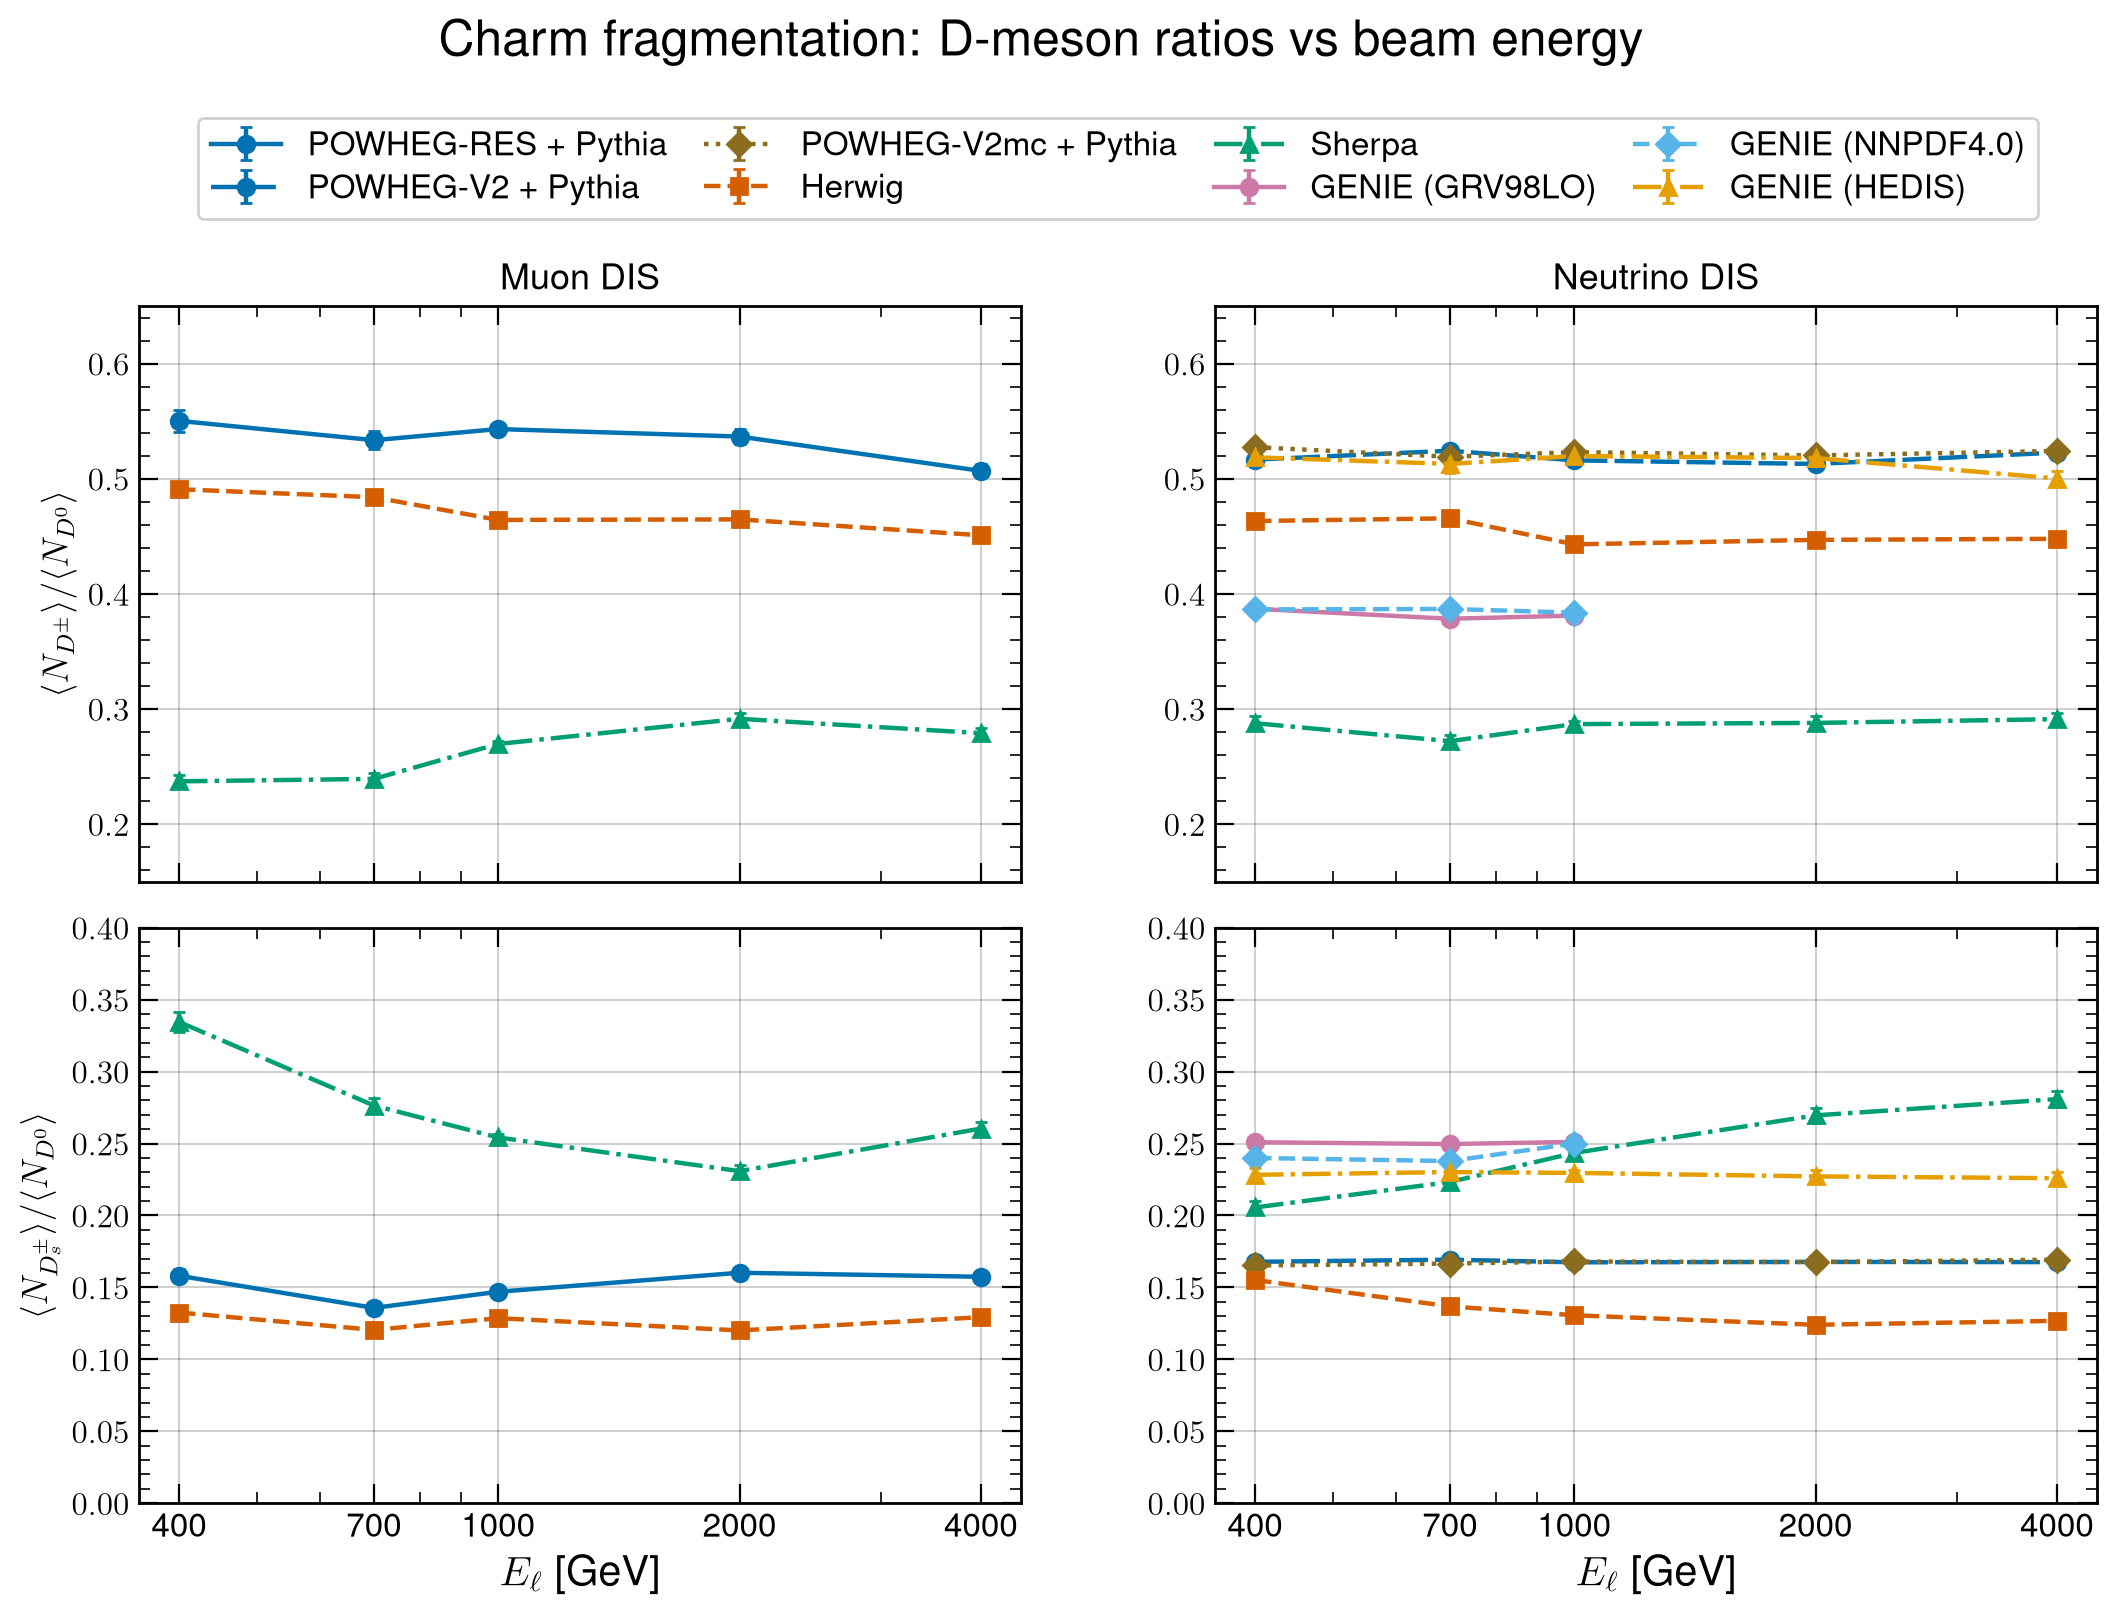
\includegraphics[width=0.94\textwidth]{figures/pp_dmeson_ratios.png}
  \caption{The ratios $\langle N_{D^\pm}\rangle/\langle N_{D^0}\rangle$ (top) and $\langle N_{D_s^\pm}\rangle/\langle N_{D^0}\rangle$ (bottom) between different $D$-meson species in charm-tagged events on tungsten as a function of the beam energy, for muon (left) and neutrino (right panels) DIS evaluated in the same fiducial region as Fig.~\ref{fig:charm-vs-energy}.
    %
    $D$-mesons from the decays of excited states, such as $D^*\to D\pi$, are also included.
    %
    The predictions for \genie are shown only for neutrino DIS. 
    }
  \label{fig:dmeson-ratios}
\end{figure}
%%%%%%%%%%%%%%%%%%%%%%%%%%%%%%%%%%%%%%%%%

\paragraph{Differential distributions.}
%
Fig.~\ref{fig:charm-distributions} presents the DIS differential distributions in $x_{\rm Bj}$, $E_h$ and $Q^2$, in the same format as Fig.~\ref{fig:dis-distributions}, for charm-tagged events, for the same calculations displayed at the fiducial level in Fig.~\ref{fig:charm-vs-energy}.
%
The qualitative findings of this differential comparison are similar to those at the fiducial level: in general, there is good agreement between the NLO-matched event generators and the \yadism ZM reference for neutrino DIS, and agreement within about $10\%$ for muon DIS, with larger deviations near phase-space edges; MHOUs and the NNLO $K$-factors are larger for muon DIS than for neutrino DIS; 
the purely massive (FFNS) calculation of \powhegtwomc predicts a significant suppression of the differential cross-sections as compared to the FONLL-matched one, and is reproduced by its analytical \yadism counterpart. 
%
We conclude that this benchmark comparison is also successful for differential distributions in charm production. 

%%%%%%%%%%%%%%%%%
\begin{figure}[!tbp]
  \centering
  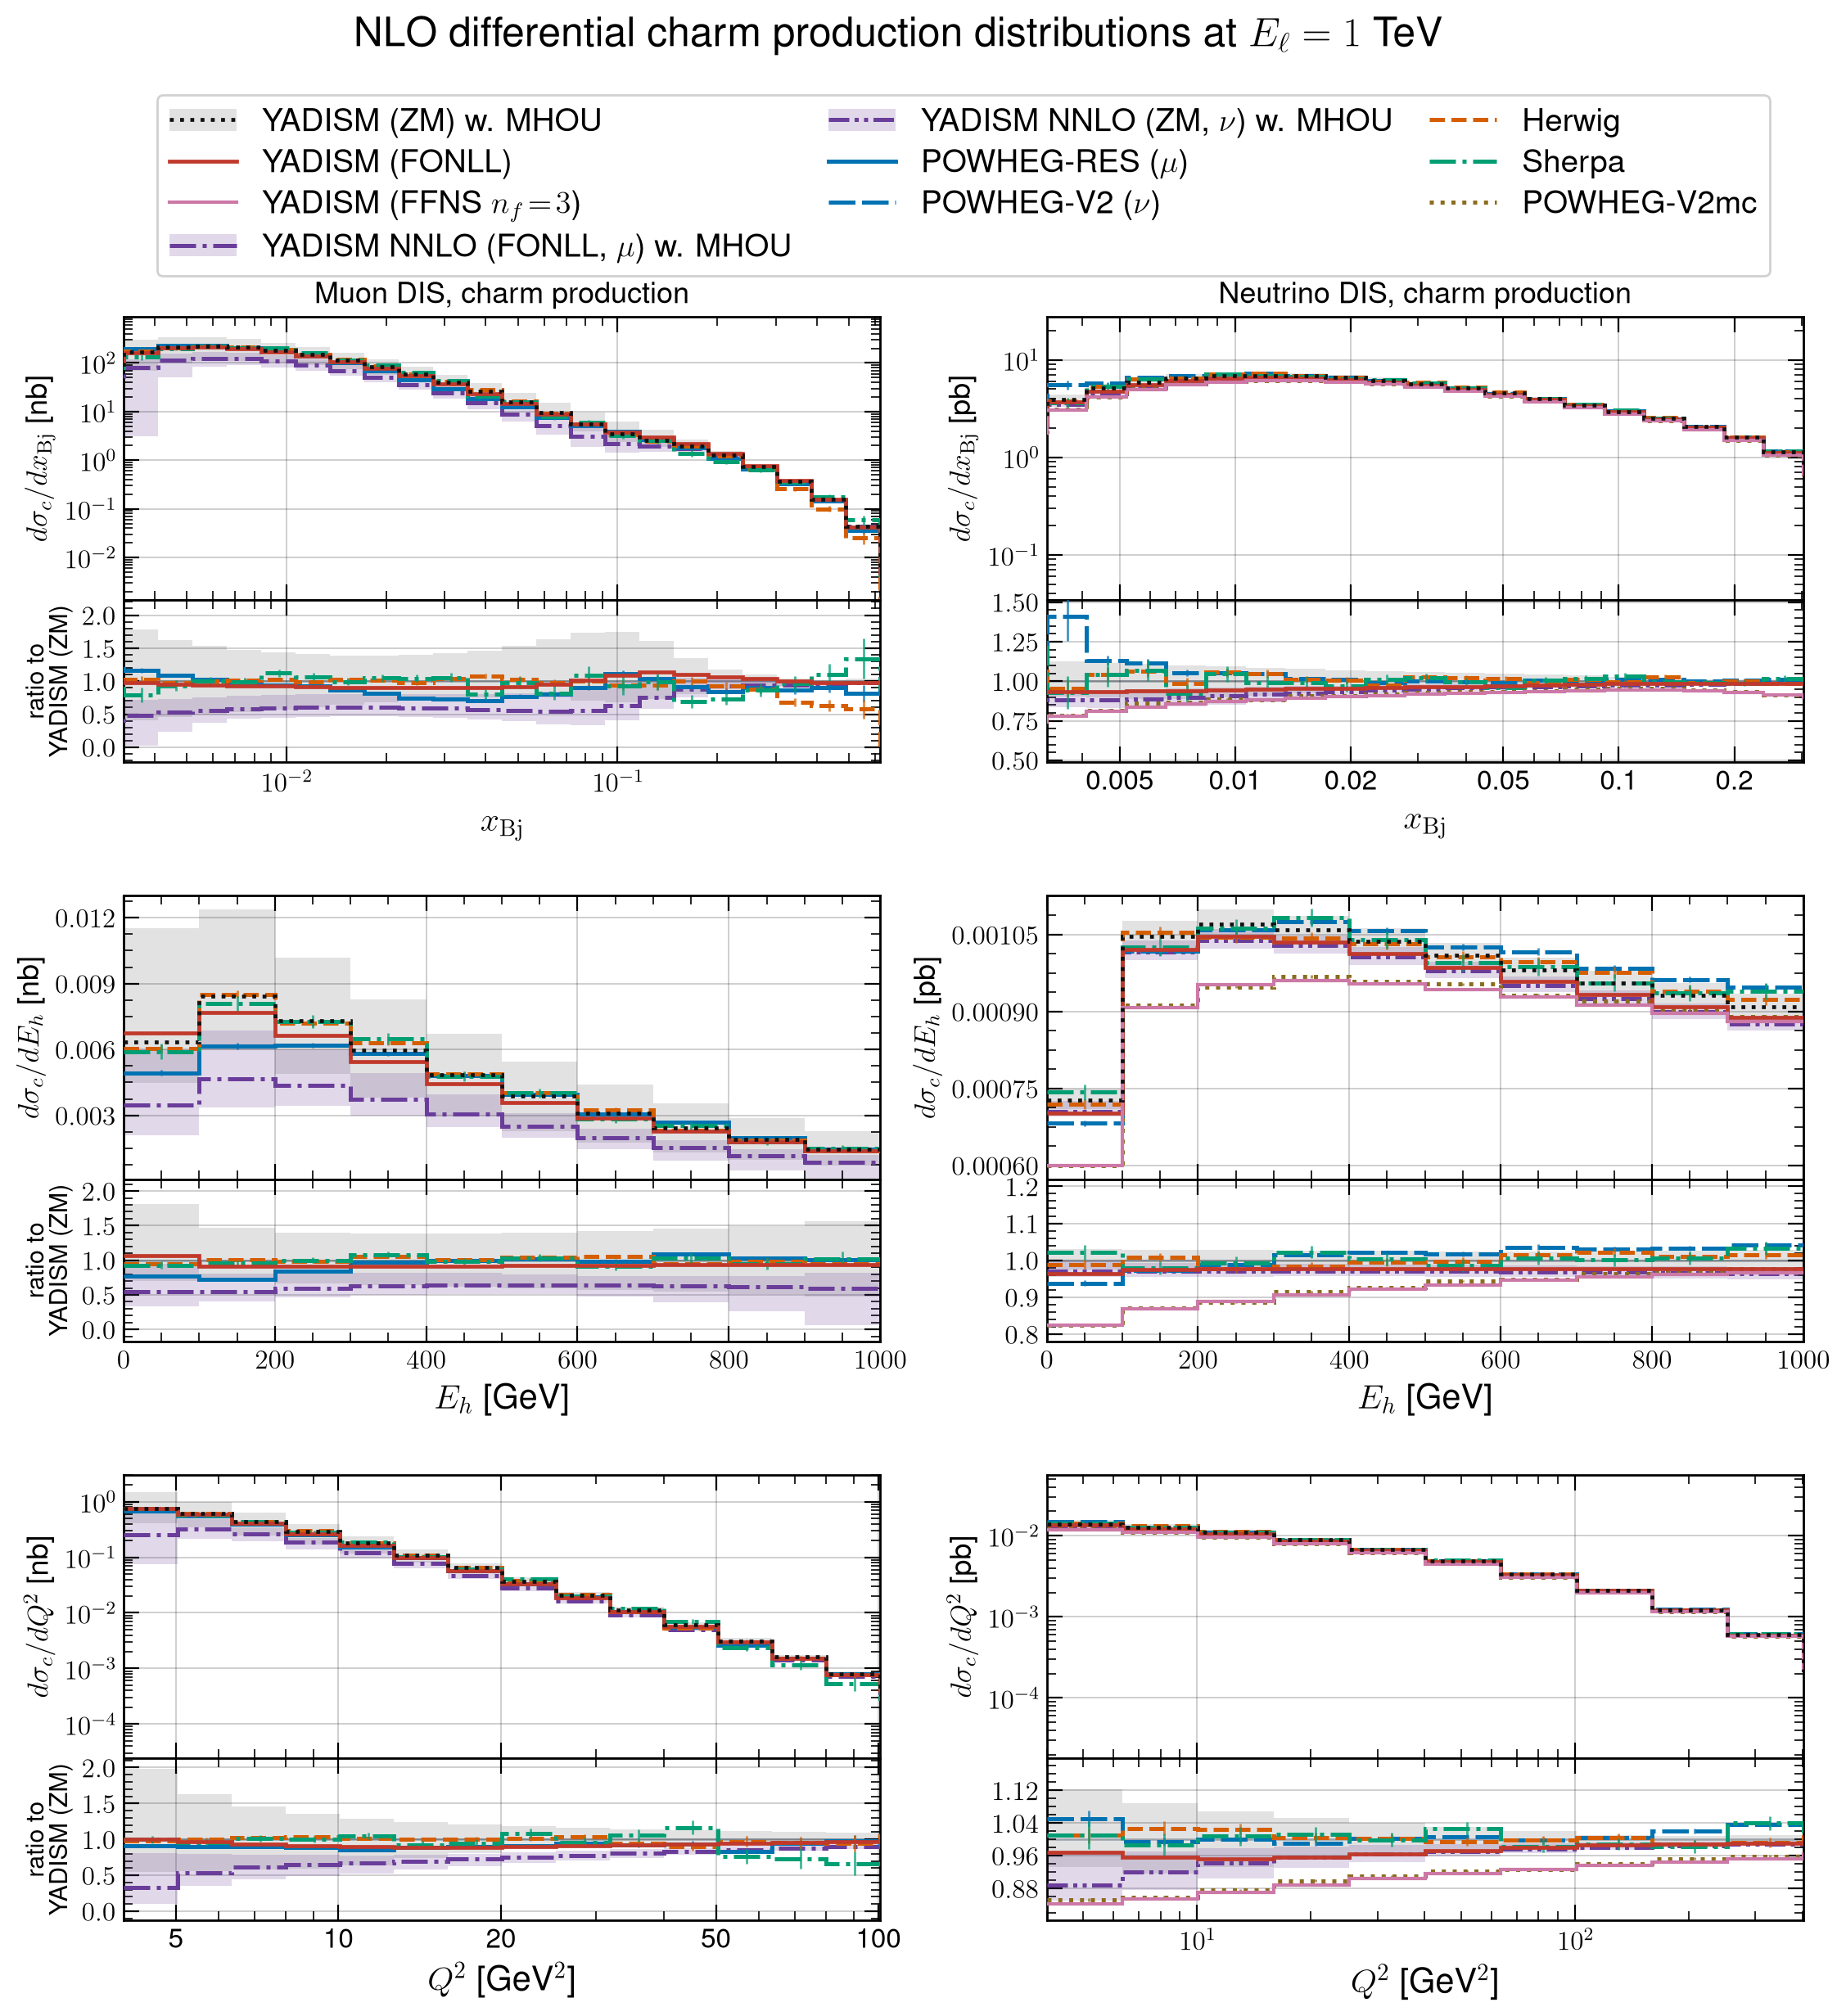
\includegraphics[width=0.99\textwidth]{figures/pp_charm_distributions.png}
  \caption{Same as Fig.~\ref{fig:dis-distributions}, now for the distributions in $x_{\rm Bj}$, $E_h$ and $Q^2$ in charm-tagged events for the same calculations displayed at the fiducial level in Fig.~\ref{fig:charm-vs-energy}.
  %
  The \yadism NNLO predictions shown are obtained in the FONLL scheme for NC DIS and in the ZM-VFNS scheme for CC DIS.
  }
  \label{fig:charm-distributions}
\end{figure}
%%%%%%%%%%%%%%%%%%%%%%%%

Finally, Fig.~\ref{fig:genie-charm-distributions} displays the same comparison for the DIS differential distributions as in Fig.~\ref{fig:charm-distributions} now including the \genie configurations, see Fig.~\ref{fig:genie-charm-vs-energy} for the corresponding predictions at the fiducial level.
%
From this comparison, we see that the deficit in the default \genie tune is not only a normalisation but also a shape effect, and is more marked at small $Q^2$ and small $x_{\rm Bj}$, where the GRV98LO strange sea PDF is most suppressed relative to \nnpdf.
%
Once \genie is run with \nnpdf, everything else unchanged,  the agreement improves but some differences remain, such as the tilt in the $E_h$ distribution, as a consequence of the charm production model adopted by \genie which predicts different yields as compared to the exact NLO QCD calculation. 
%
As was already the case for fiducial cross-sections, also at the differential level \powhegtwomc reproduces the \yadism FFNS $n_f=3$ calculation to within $3\%$.

%%%%%%%%%%%%%%%%%%%%%%%%%%
\begin{figure}[!tbp]
  \centering
  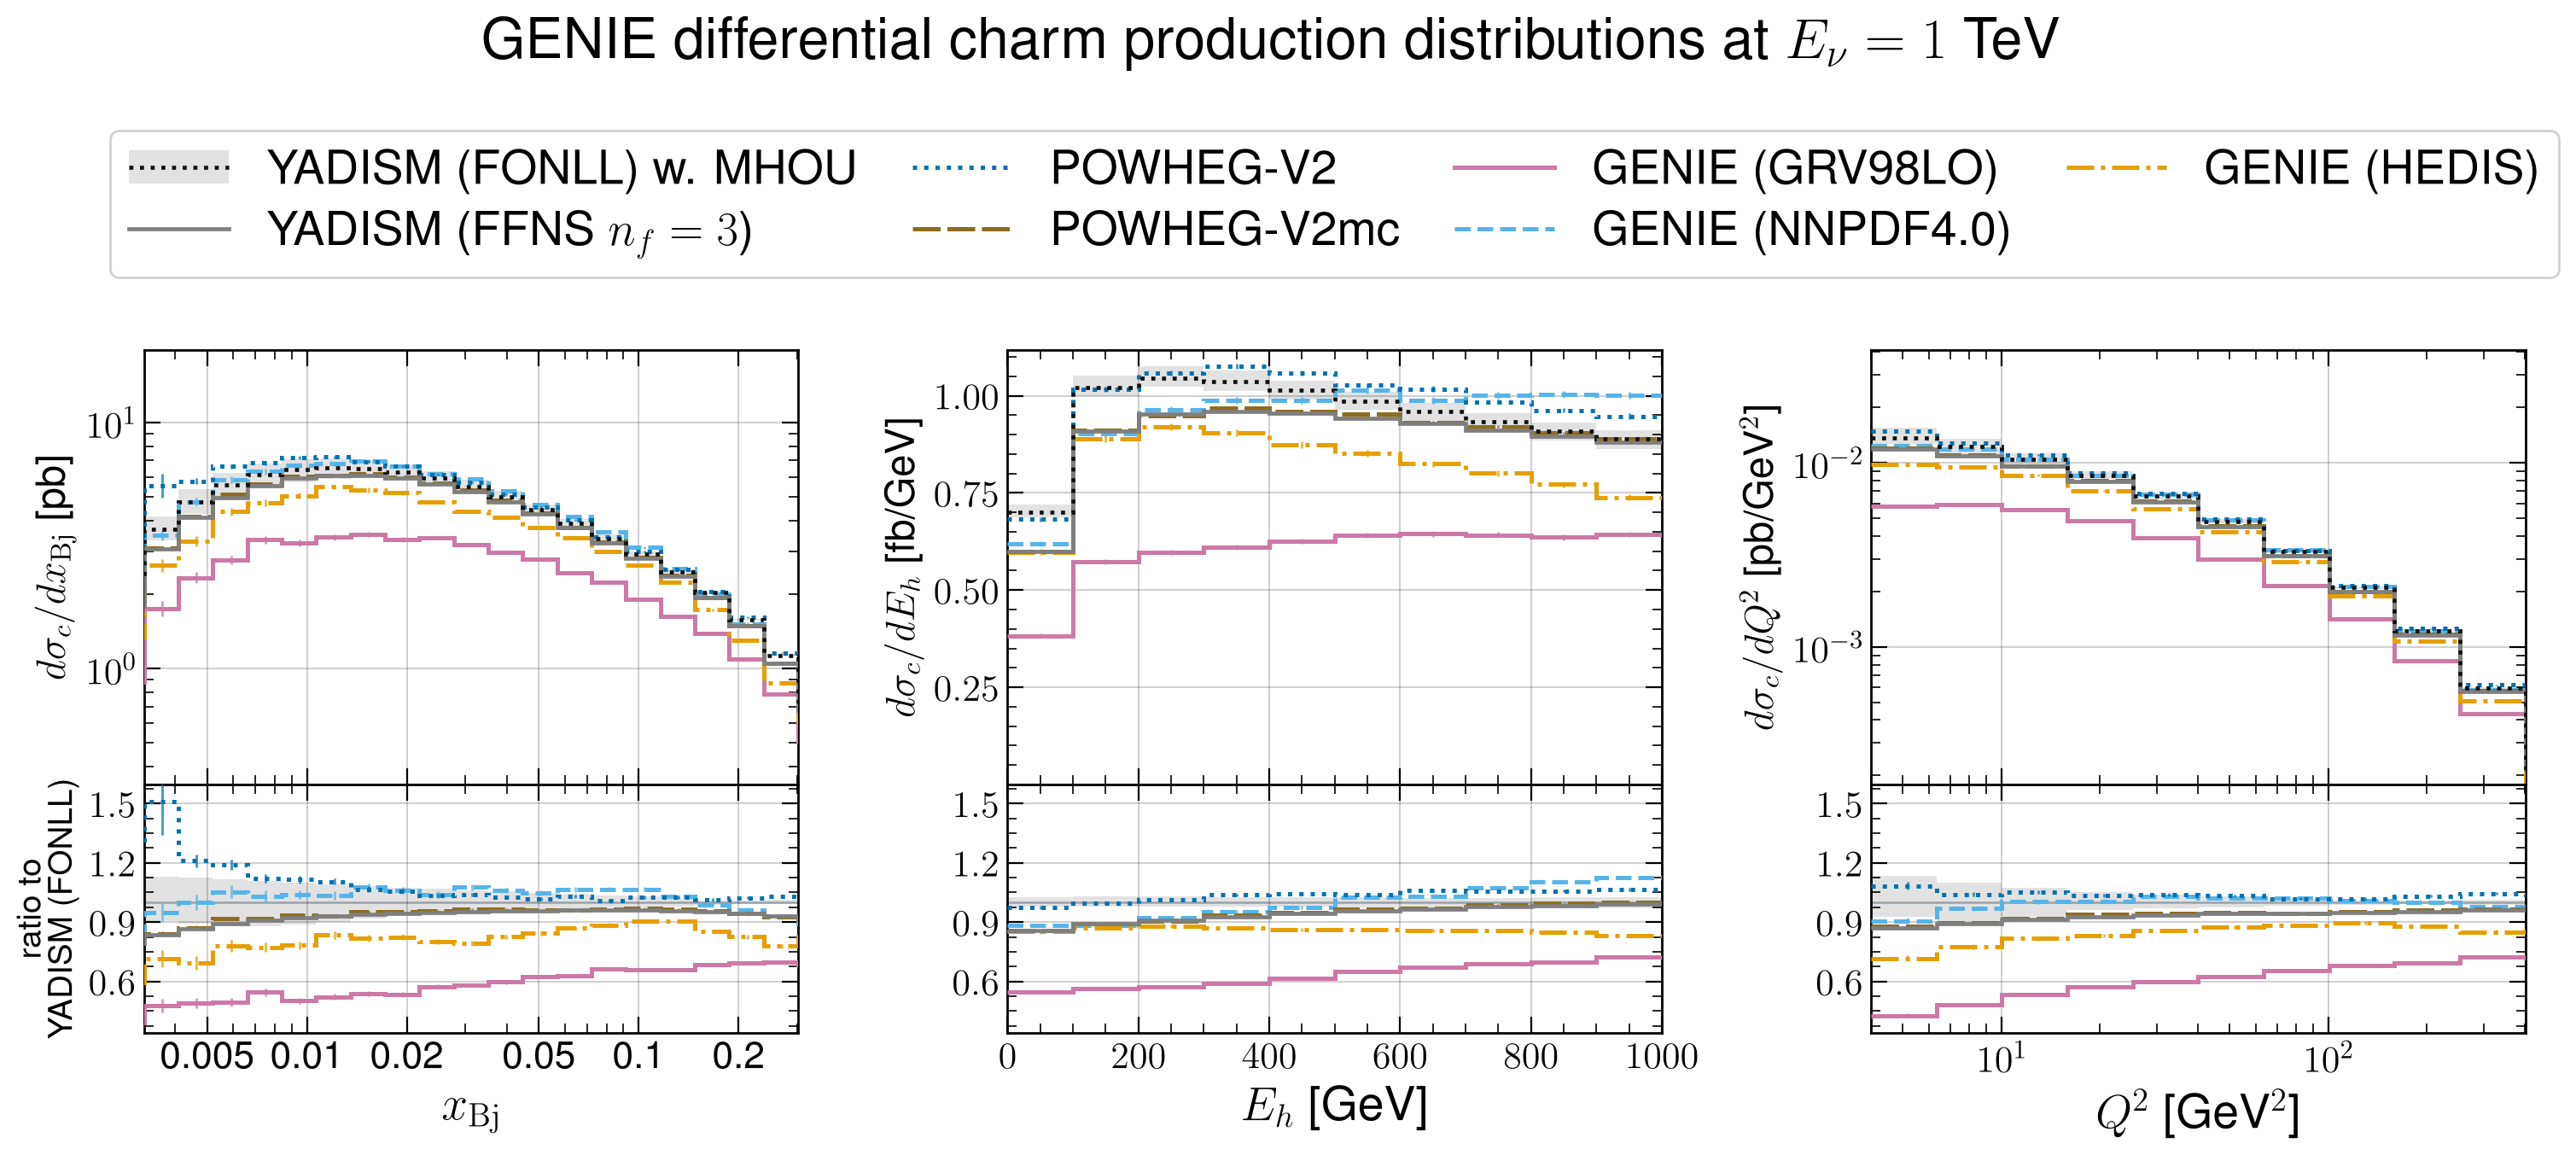
\includegraphics[width=0.99\textwidth]{figures/pp_genie_charm_distributions.png}
  \caption{Same as Fig.~\ref{fig:genie-charm-vs-energy} for the differential distributions in $x_{\rm Bj}$, $E_h$ and $Q^2$ in charm-tagged neutrino DIS events at $E_\nu=1$ TeV.
    %
    The bottom panels display the ratio to the \yadism FONLL prediction.
    }
  \label{fig:genie-charm-distributions}
\end{figure}
%%%%%%%%%%%%%%%%%%%%%%%%%%%%

